\setcounter{secnumdepth}{-1}

\chapter{Synchronization errors}

\section{Description}

Because the receiver and transmitter are not at the same location, the carrier frequencies and the samplers at TX and RX will have a different phase and due to the inaccuracies of the oscillator, the frequencies will also be slightly different. \\
This is summarized in 4 effects:
\begin{itemize}
    \item \textbf{Carrier frequency offset (CFO)}: The difference in the carrier frequencies at TX and RX ($=\Delta \omega$). It will add ISI as the RRC are not anymore matched and a linearly increasing phase shift will appear.
    \item \textbf{Phase offset}: The difference between the phase of the carrier signal at TX and RX.
    \item \textbf{Sampling frequency offset (SFO)}: The difference in the sampling frequencies at TX and RX.
    \item \textbf{Time shift}: The timing offset of the sampling at TX and RX.
\end{itemize}

\section{Implementation}

\subsection{CFO}
The CFO implementation is done by multiplying the signal with a complex exponential $e^{j2\pi \phi_{\text{ppm}}f_c t}$. The phase offset is added to the CFO. It is defined in ppm (part per million) where the ppm value is $\frac{\Delta\omega}{f_c} 10^{-6}$. \\
Figure \ref{fig:CFO_BER} shows the BER curves with different CFO values. In order to have useful results, the linear phase shift is removed right after the second RRC filter. This allows to only keep the effect of ISI on the BER curve.

\begin{figure}[H]
    \centering
    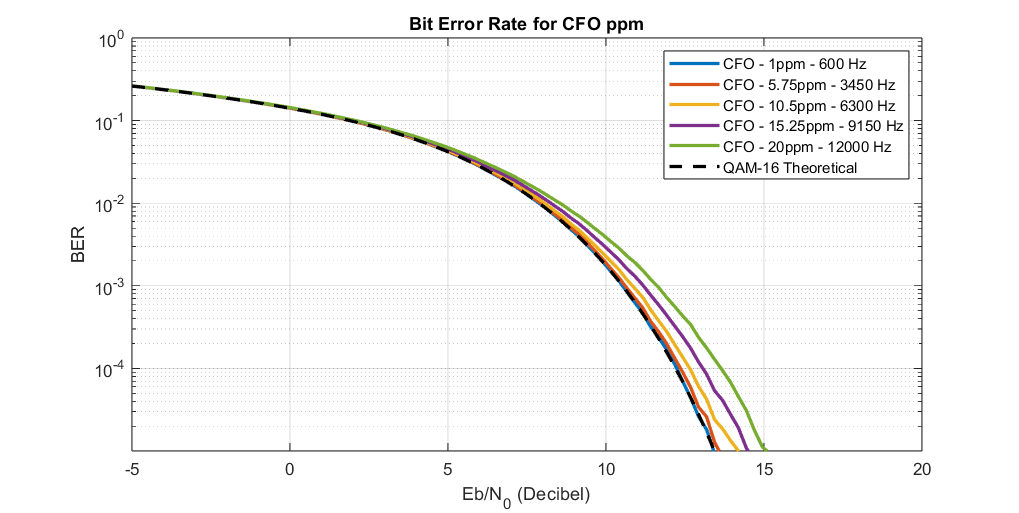
\includegraphics[width=0.8\textwidth]{CFO_ppm.png}
    \caption{BER with different CFO values}
    \label{fig:CFO_BER}
\end{figure}

Figure \ref{fig:CFO_const} shows the effect of CFO on the symbol constellation for QAM-16. The linear increase of the phase due to CFO makes the received symbols to form circles in the constellation diagram. \\

\begin{figure}[H]
    \centering
    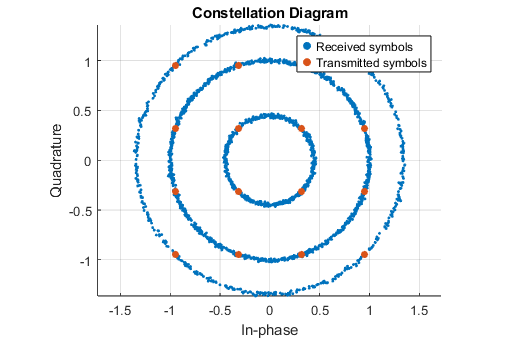
\includegraphics[width=0.8\textwidth]{constellation_CFO.png}
    \caption{Constellation before and after CFO}
    \label{fig:CFO_const}
\end{figure}

\subsection{Phase offset}
The same is done for the phase offset where the exponential is simply $e^{j\phi}$ where $\phi$ is chosen once at the begining of the simulation. \\

The effect of the phase offset is only visible on the constellation plot (figure \ref{fig:phaseOffsetConst}) where every point is rotated by a fixed angle (whereas CFO rotated the symbols linearly with time). \\

\begin{figure}[H]
    \centering
    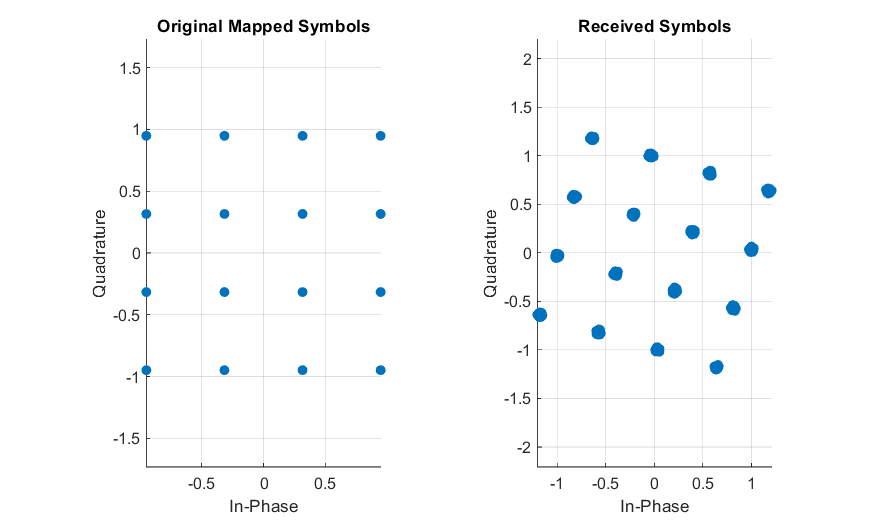
\includegraphics[width=0.8\textwidth]{constellation_carrier_offset.png}
    \caption{Constellation before and after phase offset}
    \label{fig:phaseOffsetConst}
\end{figure}

On a BER curve (figure \ref{fig:BER_PO}), the phase is not visible as from the errors originating from the phase offset are either on every symbol or on none and this is why the error does not depend anymore on $E_b/N_0$. \\

\begin{figure}[H]
    \centering
    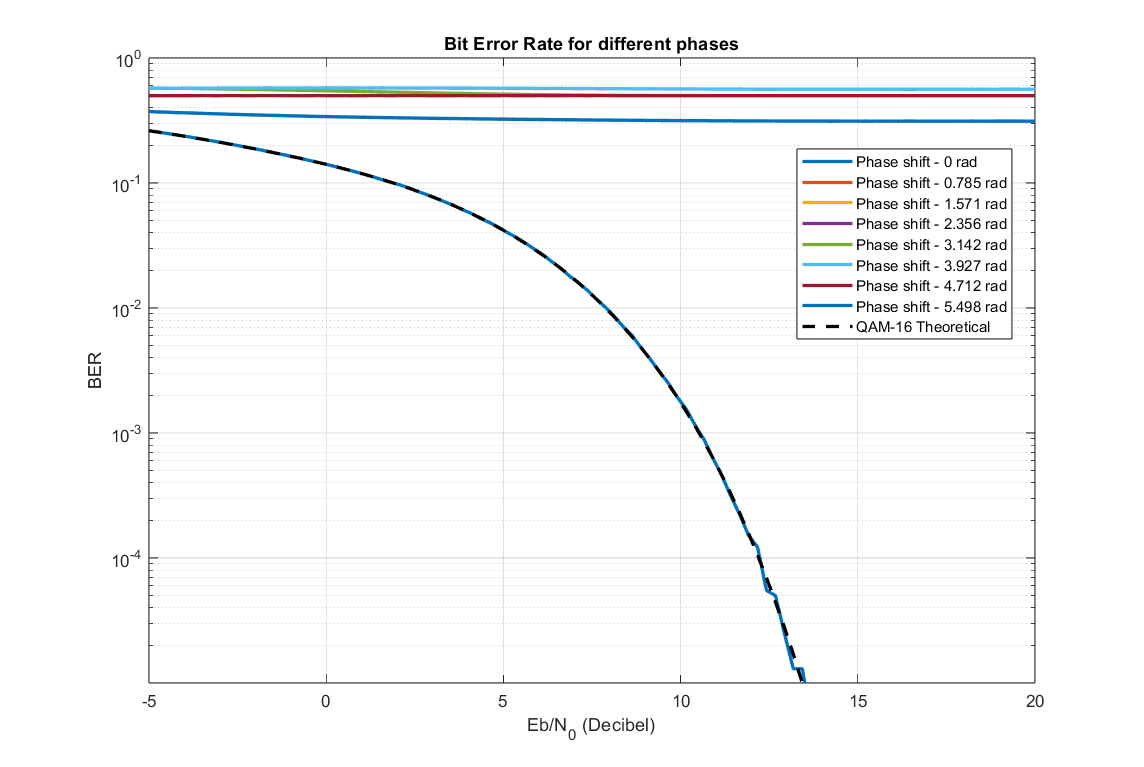
\includegraphics[width=0.8\textwidth]{BER_PO.png}
    \caption{BER with phase offset}
    \label{fig:BER_PO}
\end{figure}

\subsection{SFO}
The SFO is neglected in the simulation as it would need some interpolation and more complex computations. \\

\subsection{Time shift}
The time shift is implemented by simply shifting the samples in the array with an oversampling factor that is large enough. \\
A larger time shift will increase the BER as the samples will be taken at the wrong time. For sufficiently low values, it will still behave as a "classical" BER curve but from some point, there is just no more correlation between the measured sample and the received one and the BER tends to a $0.5$ line, as shown in figure \ref{fig:BER_TS}. \\

\begin{figure}[H]
    \centering
    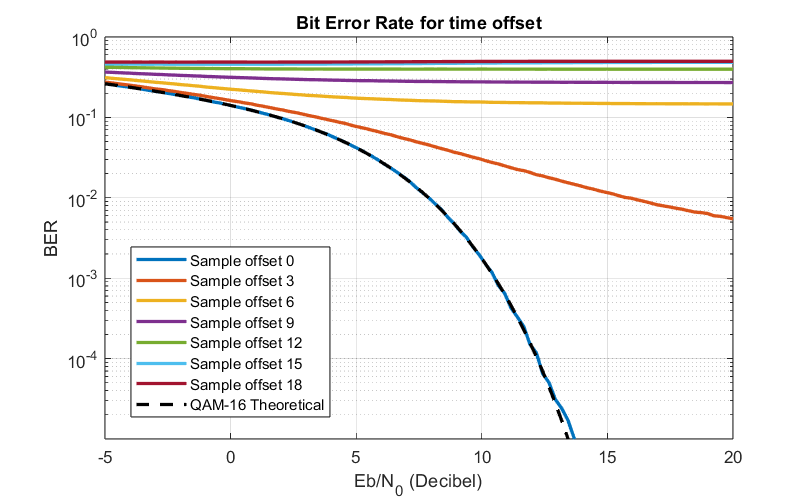
\includegraphics[width=0.8\textwidth]{BER_TS.png}
    \caption{BER with time shift}
    \label{fig:BER_TS}
\end{figure}

As the phase offset makes the receiver sample the signal between true symbols, the constellation at its output has points that are spread around the initial symbols, as shown in figure \ref{fig:phaseShiftConst}. 

\begin{figure}[H]
    \centering
    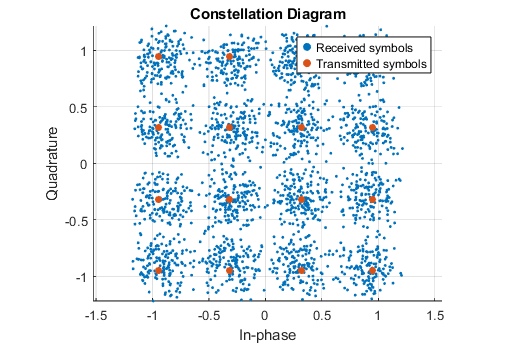
\includegraphics[width=0.6\textwidth]{constellation_timeOffset.png}
    \caption{Constellation diagram with a phase offset of 15\% of the symbol period}
    \label{fig:phaseShiftConst}
\end{figure}

\subsection{Choice of $E_{b}/N_{o}$}
Securing a SNR high enough to ensure a remaining acceptable time error after Gardner algorithm implementation
 (2 percents of the symbole rate) is a necessary condition to fulffill.\\
The impact on the BER can be seen on the graph below - figure \ref{fig:time_shift_error_SNR}.
In our case, for a symbol rate of 5MHz, the SNR should be above 4dB - 5dB by referring to the simulation plots projected 
during the course of Professor Horlin.

\begin{figure}[H]
    \centering
    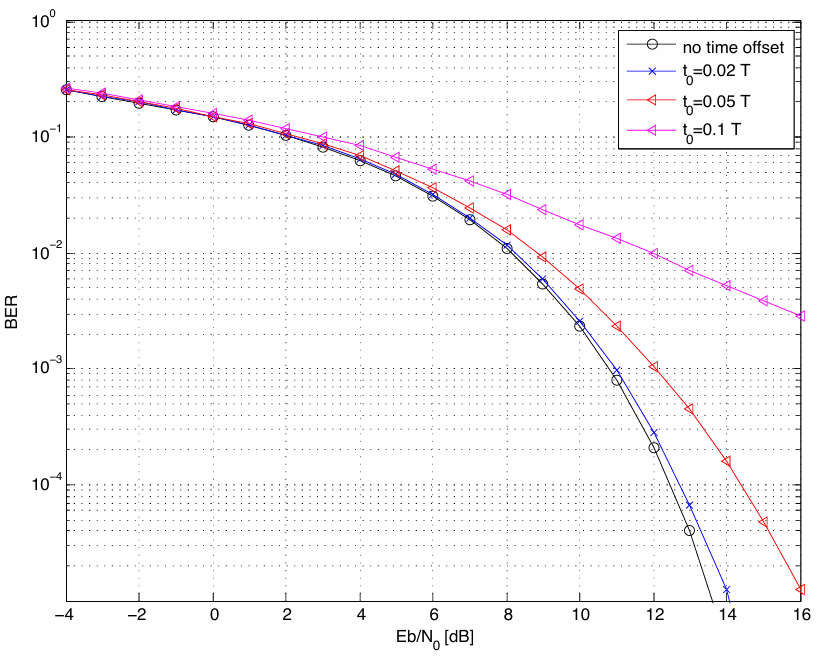
\includegraphics[width=0.7\textwidth]{time_shift_error_SNR.png}
    \caption{Impact of time shift on bit error rate}
    \label{fig:time_shift_error_SNR}
\end{figure}

To confirm this assumption, we run Gardner algorithm for different SNR values in order to confirm the remaining time shift after
Gardner.  The result is plotted in the figure \ref{Time_Shift_SNR} for 2500 symbols and a bandiwth of 5MHz.
Figure \ref{Time_Shift_evolution_SNR} shows the time shift estimation evolution for different SNR and 2500 symbols. 
 One can notice that the remaining time shift drops below 1.5\% of the symbol rate from a SNR of 4dB which is inline with what 
 was expected from the result shown during the course of Modulation and Coding.  For the remaining tasks, a SNR of 5dB will be 
 used as safety margin.
Morevover, this SNR allows us to achieve, once the frame synchronisation implemented, a remaining carrier frequency offset
of 2 ppm which is very close from the BER performance we can get without CFO - figure \ref{fig:carrier_shift_error_SNR}.

\begin{figure}[H]
    \centering
    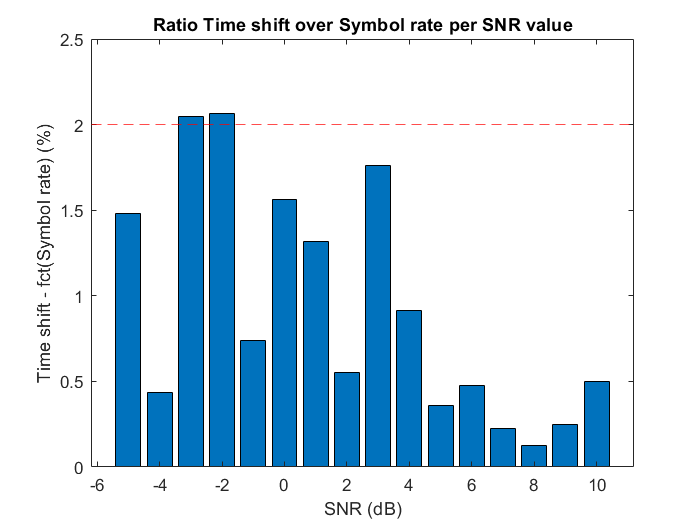
\includegraphics[width=0.7\textwidth]{Time_Shift_SNR.png}
    \caption{Remaining time shift after Gardner expressed in symbol rate percentage}
    \label{Time_Shift_SNR}
\end{figure}

\begin{figure}[H]
    \centering
    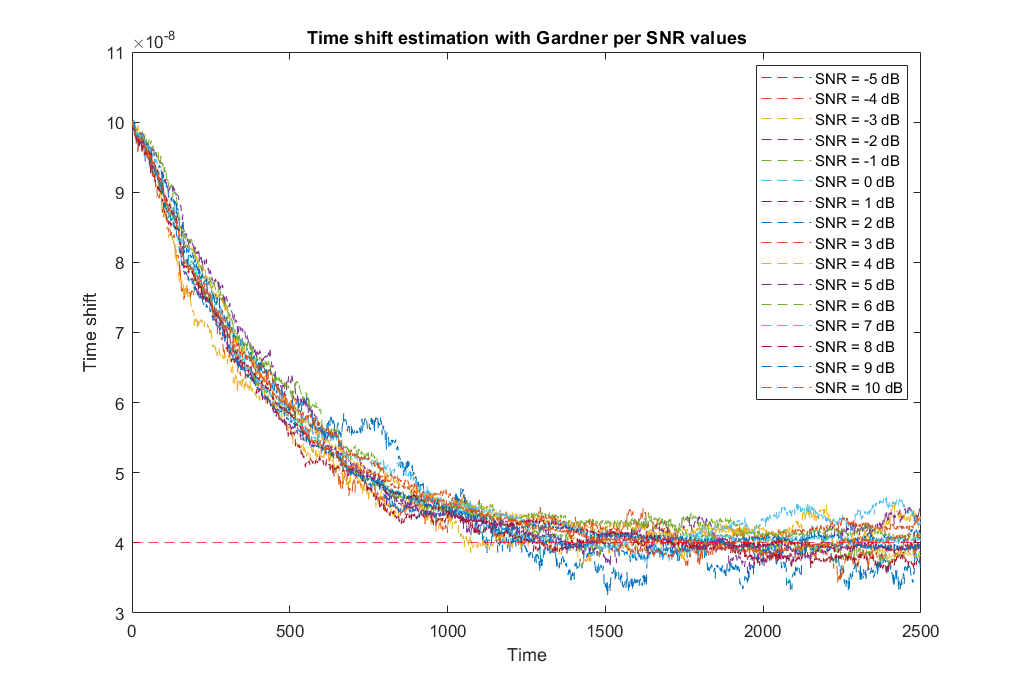
\includegraphics[width=0.9\textwidth]{Time_Shift_evolution_SNR.png}
    \caption{Gardner Algorithm : Time shift evolution per different SNR values}
    \label{Time_Shift_evolution_SNR}
\end{figure}


\begin{figure}[H]
    \centering
    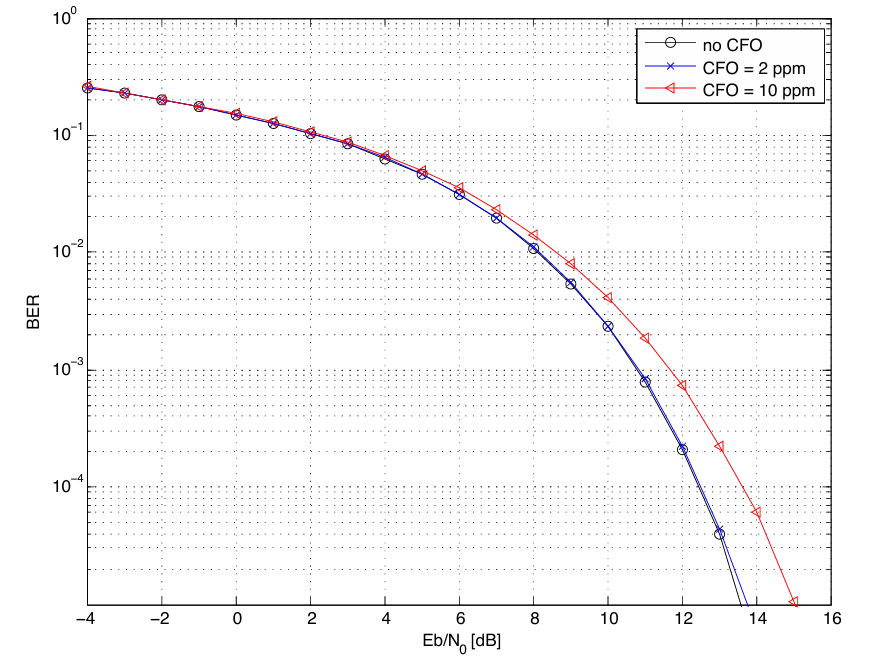
\includegraphics[width=0.8\textwidth]{carrier_shift_error_SNR.png}
    \caption{Impact of carrier frequency offset on bit error rate}
    \label{fig:carrier_shift_error_SNR}
\end{figure}

\subsection{Length of the pilot and the data sequence}

Another condition to successfully implement the frame synchronisation algorithm and secure a remaining 
CFO of 2 ppm, for a SNR of 4-5dB, is to ensure to get:
\begin{itemize}
    \item A preamble with a large enough number of symbols (N>20).
    \item Cross-correlation sub-windows which are enough separated (K>8).  
\end{itemize}

\section{Correction}

\subsection{Synchronisation error correction order}

The main bottleneck of the synchronisation error correction is the combination of the time shift error and
 the carrier frequency error.
This error combination leads us to model an algorithm which correct one whithout being affected by the other.
The Gardner algorithm is fulfilling this condition as it is able to correct the time shift error and is also robust to CFO.
Once the time shift error is corrected, the second algorithm can be implemented and detect/estimate the frequency shift introduced by the CFO.\newline

The results of the implementation of this Gardner algorithm for different time shifts and different weight coefficients \textbf{k} are plotted below
showing the performance of the coded algorithm inline with what was expected.

\begin{figure}[H]
    \centering
    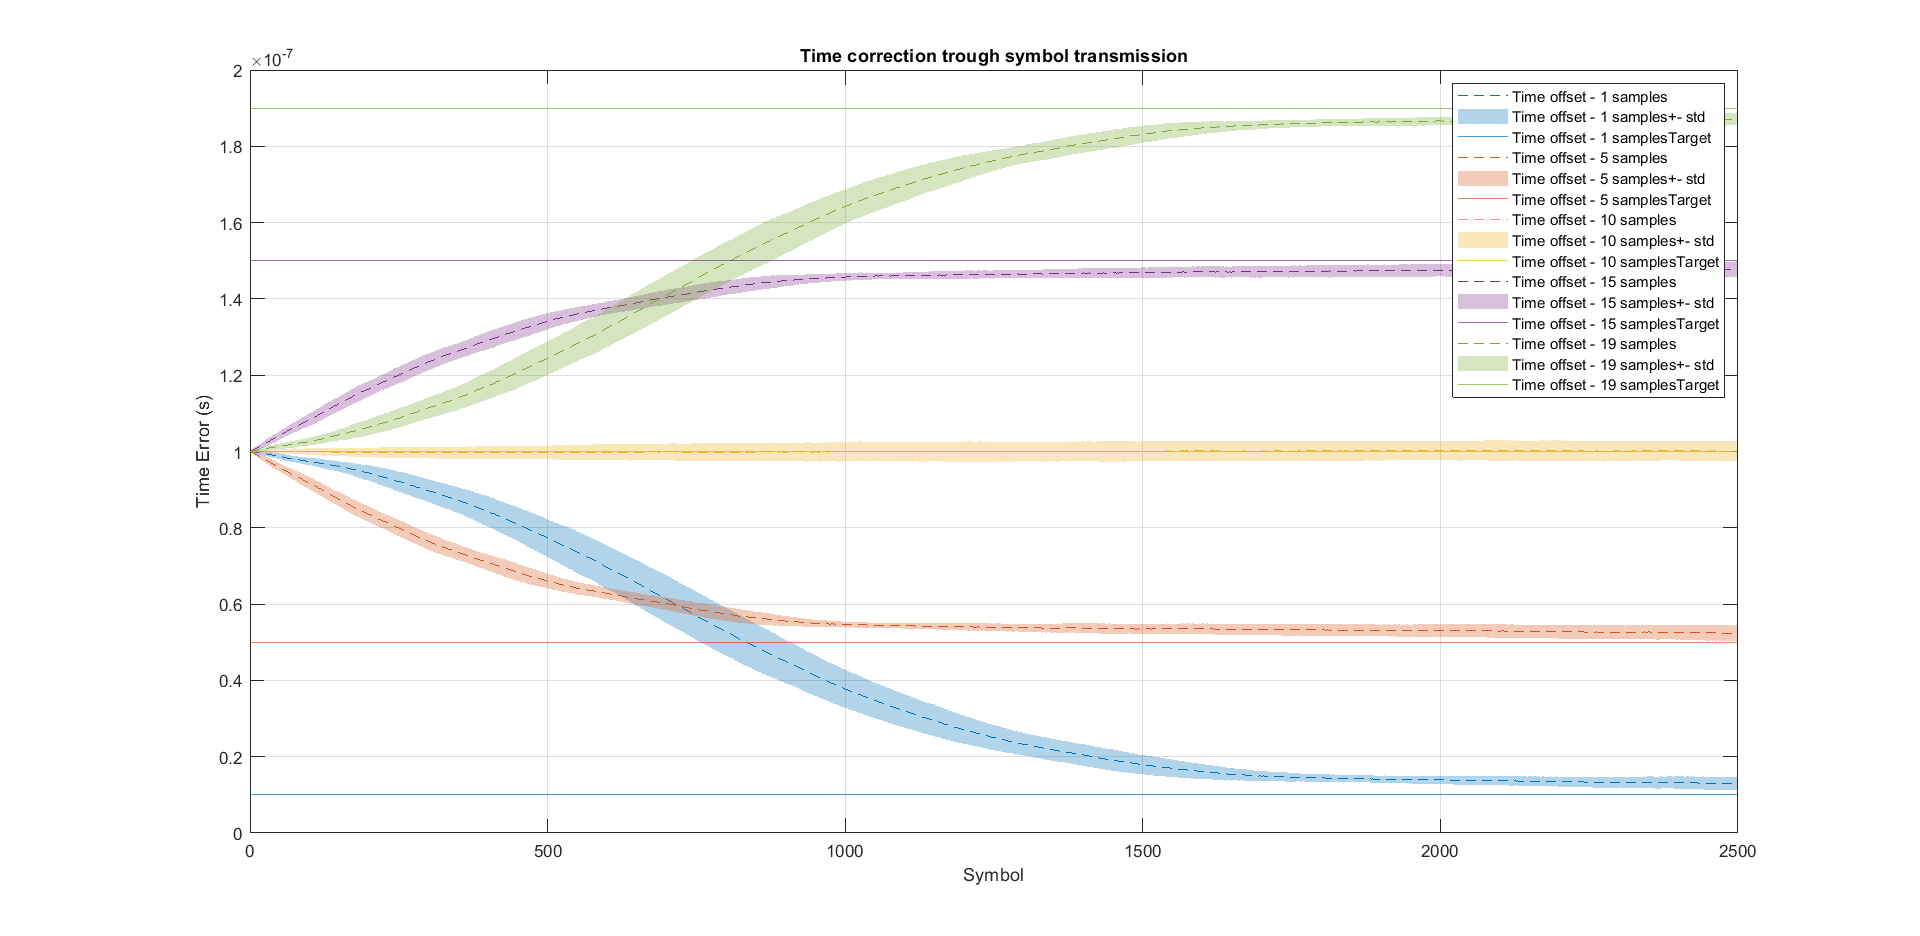
\includegraphics[width=1\textwidth]{Gardner_time_error_correction.png}
    \caption{Time offset estimation over the samples with different time shifts}
    \label{fig:Gardner_time_error_correction}
\end{figure}

\begin{figure}[H]
    \centering
    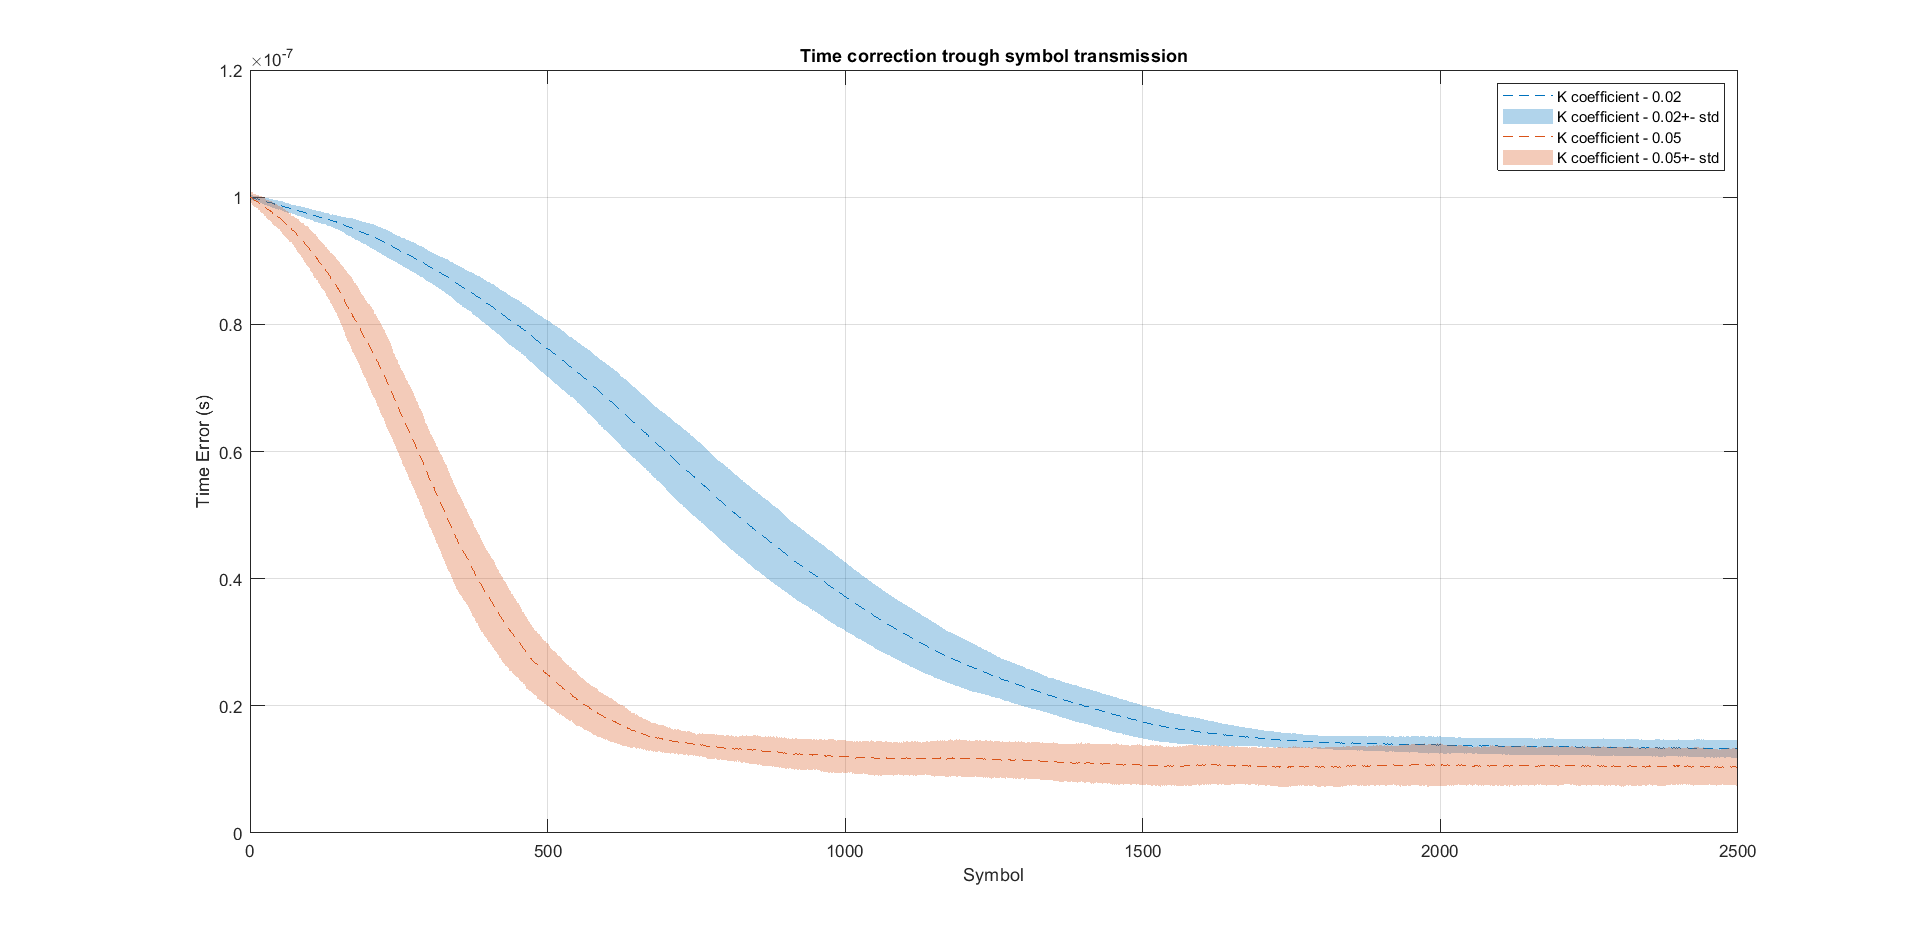
\includegraphics[width=1\textwidth]{Gardner_weigthed_coefficient.png}
    \caption{Time offset estimation over the samples with different weight coefficients}
    \label{fig:Gardner_weigthed_coefficient}
\end{figure}

It is also interesting to mention that the Gardner algorithm is a \textbf{continuous} error correction - which means that
the time shift error is corrected along the symbol stream sent.\\
In the other hand, The frame synchronisation is a correction done by analyzing a \textbf{window} of symbols.

\subsection{CFO robustness of the Gardner algorithm and error interpolation}

To understand why the Gardner algorithm is robust to CFO, we would need to analyze mathematically the algorithm:

\begin{equation*}
    \epsilon_{n+1} = \epsilon_{n} - \frac{2k}{T} R[y_{\epsilon_{n}}[n-\frac{1}{2}](y_{\epsilon_{n}}^{*}[n] - y_{\epsilon_{n-1}}^{*}[n-1])]
\end{equation*}

By taking a close look to the equation, one can observe that the error is corrected by taking the midpoint and multiplying the difference between 2 adjacent symbols (which is why the algorithm is
continuous). This specificity limits the effect of a phase shift.  Indeed, multiplying the midpoint with the complex conjugates of 2 adjacents points results to 
a difference of terms of opposite rotation with negligibe phase impact for realistic CFO value.  Thus, leading to Gardner algorithm being robust to CFO.\newline
It should be mentionned that the Gardner algorithm is used with an interpolation function as the time error calculated per symbol 
may not fall accurately to a time sample bin.  Therefore, it would be wise to oversample the symbol stream judiciously to compute an 
accurate time error after interpolation.

\subsection{Differential cross-correlation}

Let's have a closer look to the cross correlation equation to grasp the intuition behind the need to use the differential cross-correlation.

\begin{equation*}
    \sum_{l}{y^{*}_{n+l}a_{l}} = \sum_{l}{I^{*}_{n+l}a_{l}e^{-j\phi_{o}}e^{-j\Delta w(n+l)T}}
\end{equation*}

We can observe that the CFO term is increasing with \textbf{l+n} resulting to a cross correlation equals to 0 even if the preamble is fitting
the window.

Therefore, the idea behind the usage of the differential cross correlation is to remove the dependency of the phase shit with \textbf{l+n}.
This idea leads to modify the equation and multiply the correlation between $y$ and $a$ with its complex conjugate term. Indeed the exponential 
terms are cancelling and remains an exponential dependent on k, the window division term.
Therefore, by computing the differential cross correlation, the calculation will result to a peak once the preamble will match with the synchronisation
 window, function of $e^{-j\Delta wk}$ and 0 in the other cases.
 
To reply to the sub-question quoting "Isn’t interesting to start the summation at k = 0 (no time shift)?", of course the reply is no as explained above.

The robustness of the gardner algorithm implemented in our Matlab code can be seen in \ref{fig:Gardner_CFO_robustness}

\begin{figure}[H]
    \centering
    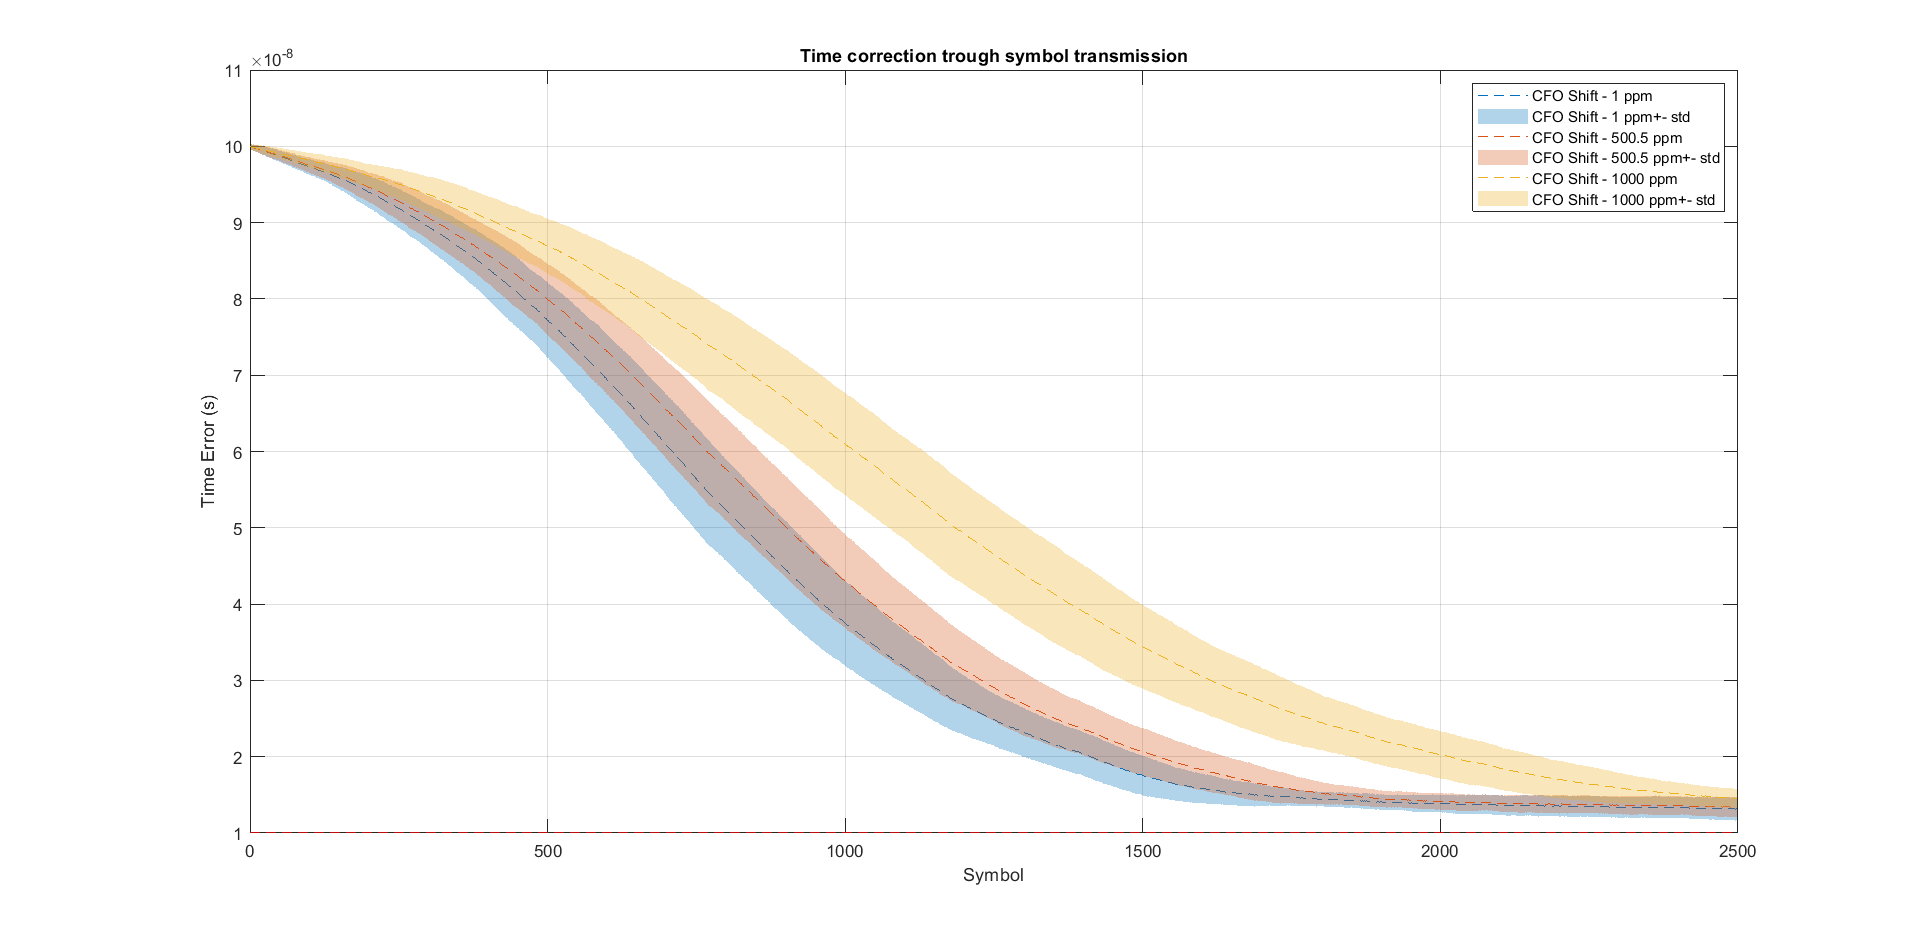
\includegraphics[width=1\textwidth]{Gardner_CFO_robustness.png}
    \caption{CFO robustness results from our Matlab code}
    \label{fig:Gardner_CFO_robustness}
\end{figure}

\subsection{Optimal criteria}

To summarize, to have a perfect frame synchronisation which means to have a frame time arrival standard deviation equals to 0 for a realistic CFO
error and a remaining time error of 2 percents at the end of Gardner module, a sine qua none condition is to get a large number of 
samples (N>20) and a large sub-division term (K>8).

\begin{figure}[H]
    \centering
    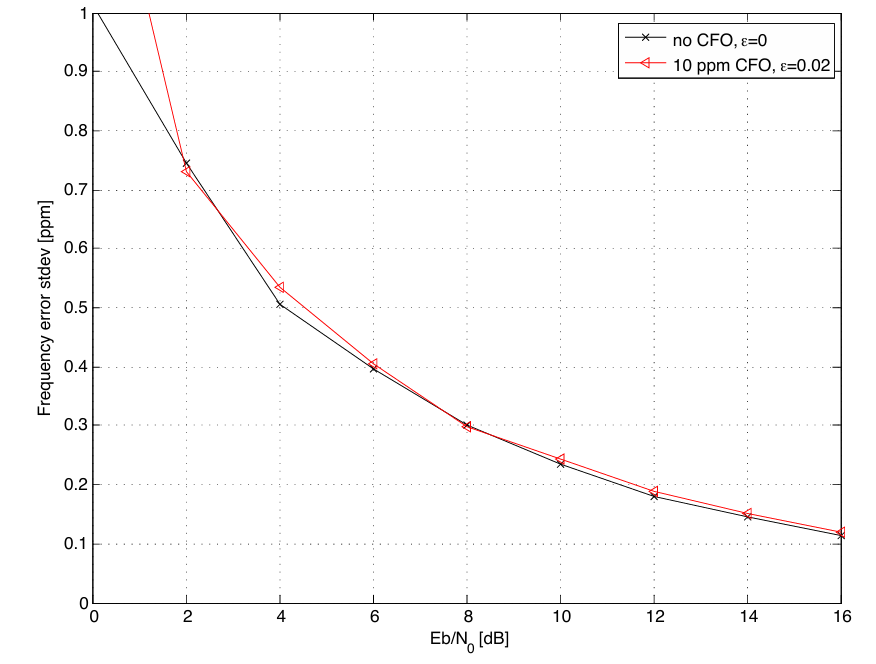
\includegraphics[width=0.8\textwidth]{time_frame_arrival_error_SNR.png}
    \caption{Frame time arrival standard deviation for realistic CFO and sampling time error based on SNR}
    \label{fig:time_frame_arrival_error_SNR}
\end{figure}
\subsection{Frame and frequency acquisition}

With the previous correction, the receiver knows when to sample but there still is some uncertainty on the frequency. The way to remove the CFO is to send in the data a known pilot and the first step is to detect when this pilot is received. This is known as frame acquisition and it is performed with the differential cross-correlator:

\begin{equation*}
    D_k[n] = \frac{1}{N-k} \sum_{l=k}^{N-1} \left(y^*[n+l]a[l]\right) \left(y^*[n+l-k]a[l-k]\right)^*
\end{equation*}

Where $a$ is the known pilot, $N$ its length and $k$ the delay between the two correlations. \\
$D_k[n]$ is computed for every time index $n$ and for every shift $k$ until its maximum value, $K$. The estimation of the index of the start of the frame $\hat{n}$ and the estimation of the CFO $\hat{\Delta f}$ are given by:

\begin{equation*}
    \hat{n} = \text{arg} \max_n \sum_{k=1}^{K} |D_k[n]|
\end{equation*}
\begin{equation*}
    \hat{\Delta f} = -\frac{1}{K} \sum_{k=1}^{K} \frac{\angle D_k[\hat{n}]}{2\pi kT}, \qquad T \text{ being the symbol duration.}
\end{equation*}

The implementation of the time of arrival estimator has been done on figure \ref{fig:TOA_demo} by placing the pilot at the 100th sample and by then plotting $\sum_{k=1}^{K} |D_k[n]|$. The peak at the 100th sample clearly indicates the time of arrival of the pilot and validates the implementation. A similar test was done for the CFO estimation but it is not shown here. \\

\begin{figure}[H]
    \centering
    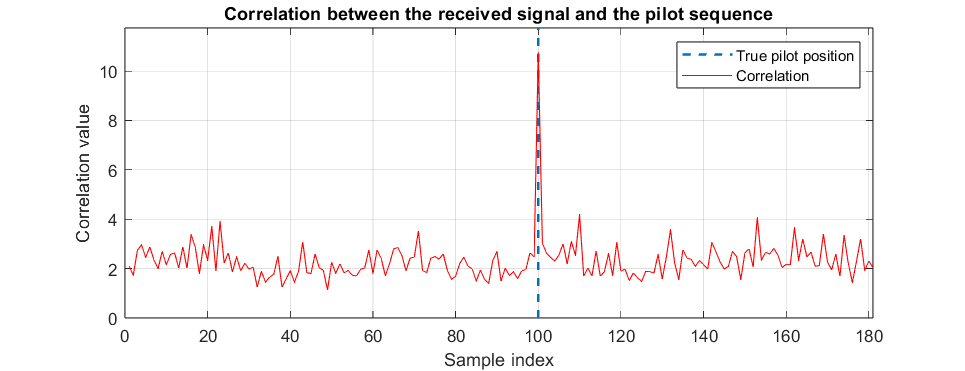
\includegraphics[width=1\textwidth]{TOA_demo.png}
    \caption{Time of arrival estimation (N=20, K=8)}
    \label{fig:TOA_demo}
\end{figure}

The standard deviation of both estimators has been mesured on 250 runs for both a varying pilot length $N$ and a varying maximal shift $K$ for an increasing $\frac{E_b}{N_0}$ in figures \ref{fig:TOA_CFO_std_N} and \ref{fig:TOA_CFO_std_K}. 

\begin{figure}[H]
    \centering
    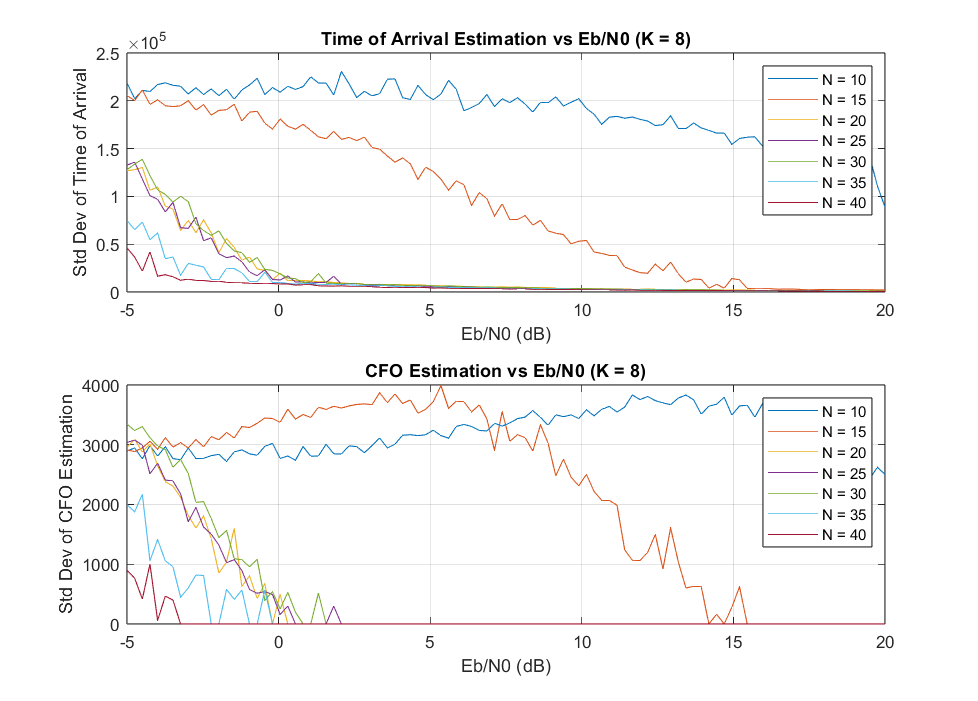
\includegraphics[width=1\textwidth]{TOA_CFO_std_56m.png}
    \caption{Standard deviation of the CFO estimator with varying pilot length}
    \label{fig:TOA_CFO_std_N}
\end{figure}

\begin{figure}[H]
    \centering
    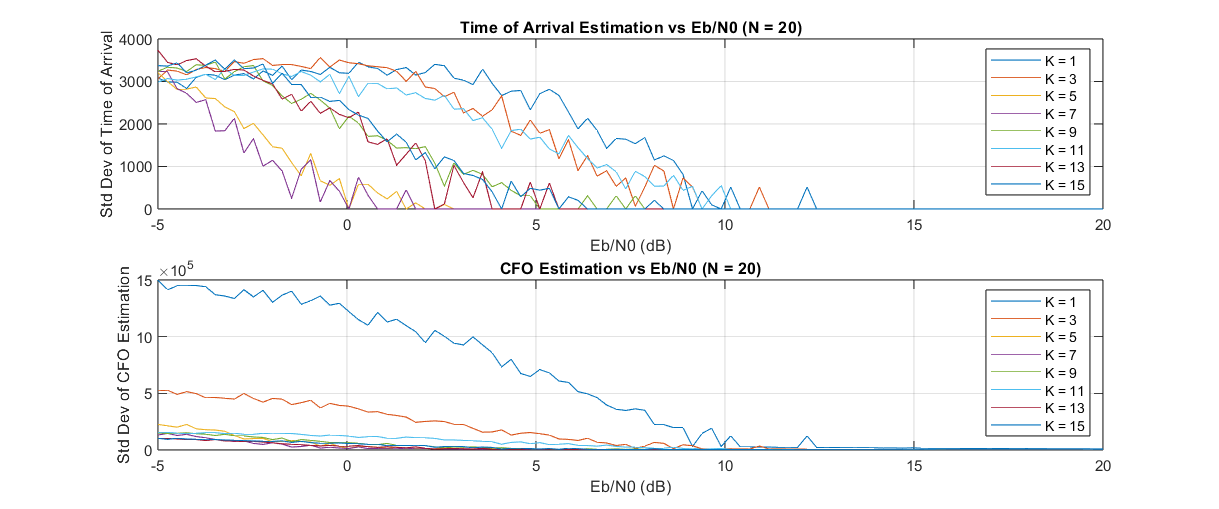
\includegraphics[width=1\textwidth]{TOA_CFO_std_K_56m.png}
    \caption{Standard deviation of the CFO estimator with varying maximal shift}
    \label{fig:TOA_CFO_std_K}
\end{figure}

As expected, a longer pilot and a larger shift will lower the uncertainty of the estimation and the same goes by for an increasing SNR. The fact that the line corresponding to $N = 10$ on figure \ref{fig:TOA_CFO_std_N} does not seem to decrease with $\frac{E_b}{N_0}$ is explained by the fact that $N$ and $K$ are too close to each other.\\
The robustness of the frame acquisition is also tested against a varying CFO by measuring the standard deviation of the time of arrival estimator for a varying CFO. The results are shown in figure \ref{fig:TOA_std_CFO} and it can be seen that the CFO has no impact on the time of arrival estimator. This is because the used algorithm is a differential cross-correlator and not a classical correlator. \\

\begin{figure}[H]
    \centering
    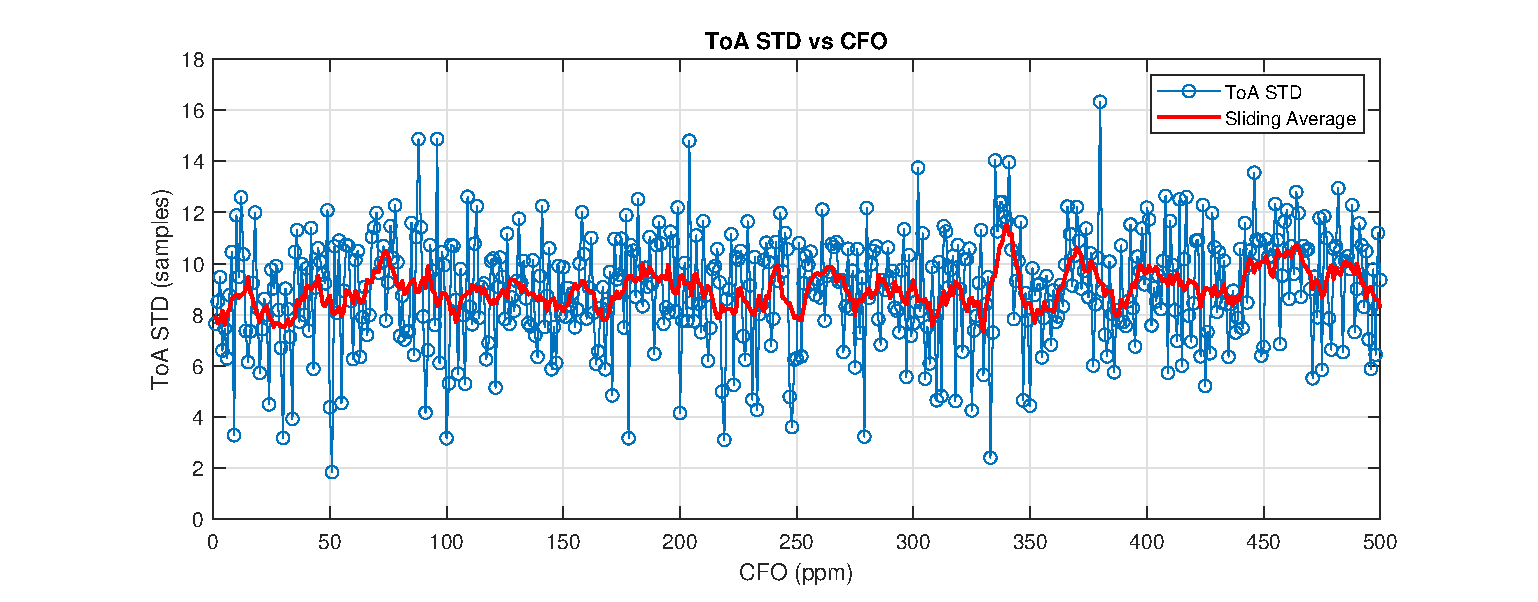
\includegraphics[width=1\textwidth]{toa_vs_cfo.eps}
    \caption{Standard deviation of the ToA estimator with varying CFO (N=20, K=8)}
    \label{fig:TOA_std_CFO}
\end{figure}

A similar test was done for the CFO estimator and the results are shown in figure \ref{fig:CFO_std_CFO}. The CFO estimator is as robust as it is based on the time of arrival estimator, which was robust to CFO. Its estimation starts to get further away from the real CFO only for unrealistic values of teh CFO. The standard deviation is pretty high, which means that a few pilots would be needed to average the estimation and have a value close to the real CFO. \\

\begin{figure}[H]
    \centering
    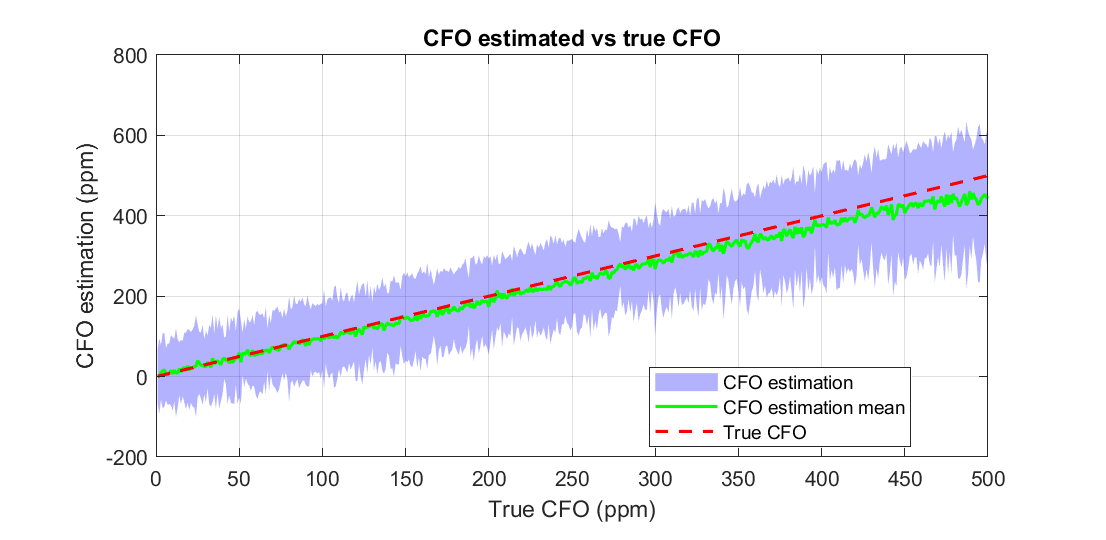
\includegraphics[width=1\textwidth]{cfo_vs_cfo.eps}
    \caption{CFO estimation with varying CFO (N=20, K=8)}
    \label{fig:CFO_std_CFO}
\end{figure}

To avoid needing a lot of pilots, the same plot was done for a higher size of the pilot and a larger shift. The results are shown in figure \ref{fig:CFO_std_CFO_N}. The standard deviation is now much lower and the estimation is still not affected by the CFO. \\

\begin{figure}[H]
    \centering
    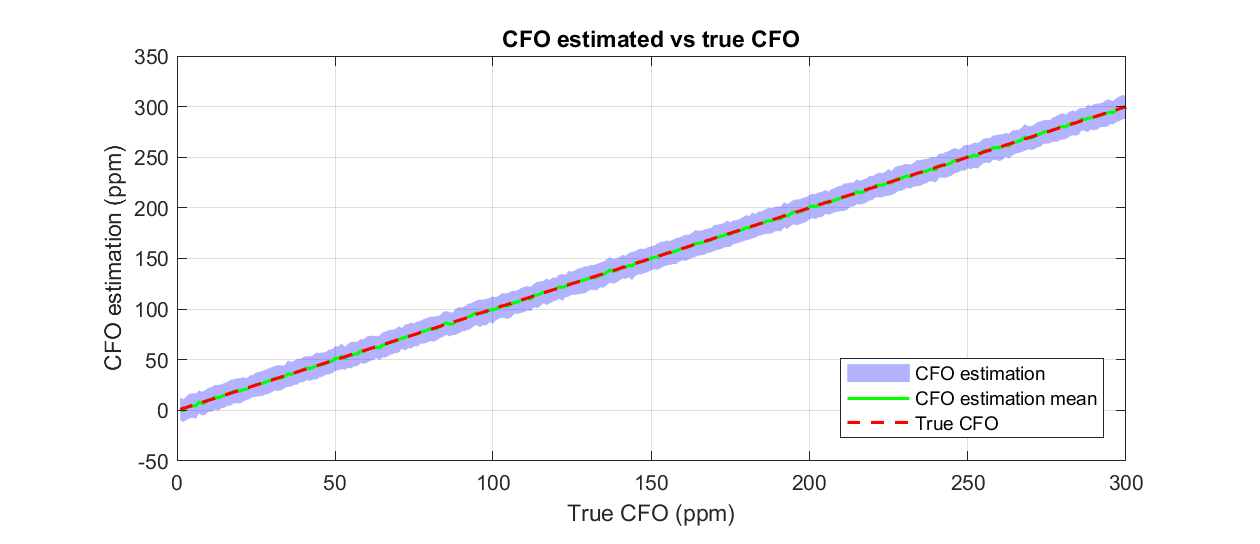
\includegraphics[width=1\textwidth]{cfo_vs_cfo_longerPilot.eps}
    \caption{CFO estimation with varying CFO (N=50, K=12)}
    \label{fig:CFO_std_CFO_N}
\end{figure}
